\documentclass[10pt,utf8]{beamer}

\mode<presentation> {
%  \usetheme{Boadilla}
  \usetheme{Madrid}
%	\usetheme{Fzu}
  \setbeamercovered{transparent}
}

\usepackage{palatino}
\usepackage{graphicx}
\usepackage{array}
\usepackage{color}
\usepackage{subfigure}
\usepackage{colortbl}
\usepackage{amsmath}
\usepackage{hyperref}
\usepackage[export]{adjustbox}
%\usepackage{tikz}
%\usetikzlibrary{arrows,shapes,backgrounds}


%\definecolor{MyDarkGreen}{rgb}{0.3,0.7,0.3}

\setbeamertemplate{caption}{\raggedright\insertcaption\par} %turn off caption prefix ("Figure")

\title{From Big Data towards Fast Data}
\author{Vojtěch Juránek}
\institute[Red Hat]{JBoss - a division by Red Hat}
\date{6.~2.~2016, DEVCONF.CZ, Brno}

\newenvironment{mylisting}
{\begin{list}{}{\setlength{\leftmargin}{1em}}\item\scriptsize\bfseries}
{\end{list}}

\newenvironment{mytinylisting}
{\begin{list}{}{\setlength{\leftmargin}{1em}}\item\tiny\bfseries}
{\end{list}}


\begin{document}

\begin{frame}
 \titlepage
\end{frame}
	
\begin{frame}
	\frametitle{Data today}
	\begin{figure}
		\centering
		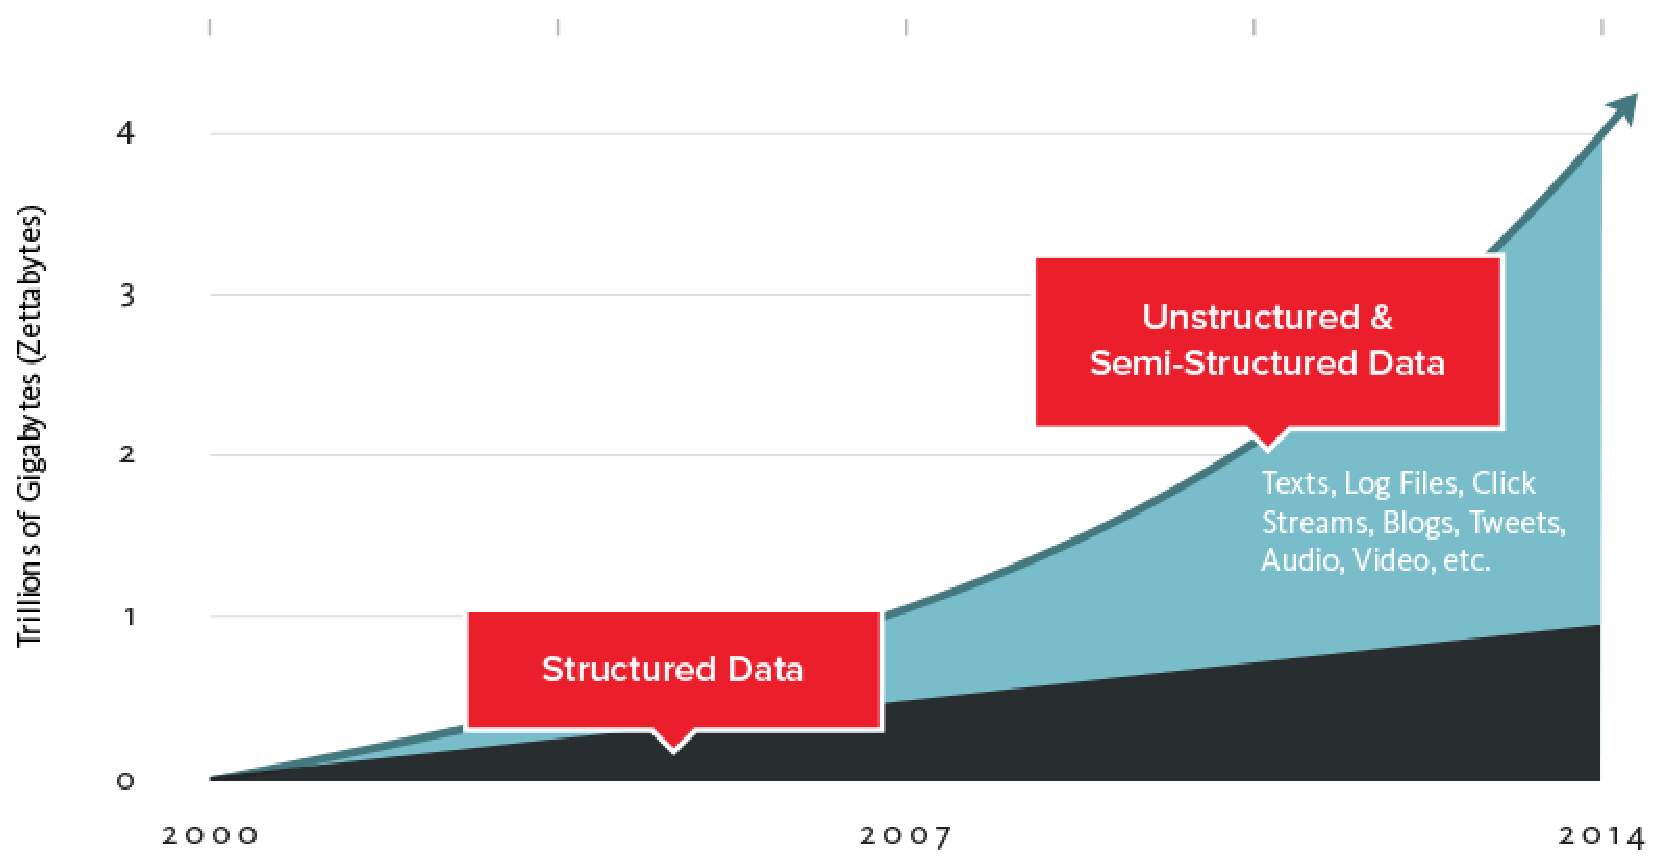
\includegraphics[width=10cm]{./img/why-nosql-2.eps}
		\caption{\tiny{Source: http://www.couchbase.com/nosql-resources/what-is-no-sql}}
	\end{figure}
	
	\vspace{-0.5cm}
	\begin{itemize}
		\item Needed ability to store unstructured data (often for performance reasons)
		\item But ability  to talk to RDBMS is often needed as well
	\end{itemize}
\end{frame}

\begin{frame}
	\frametitle{How big are Big data?}
	\visible<2,3> {
		\begin{figure}
			\centering
			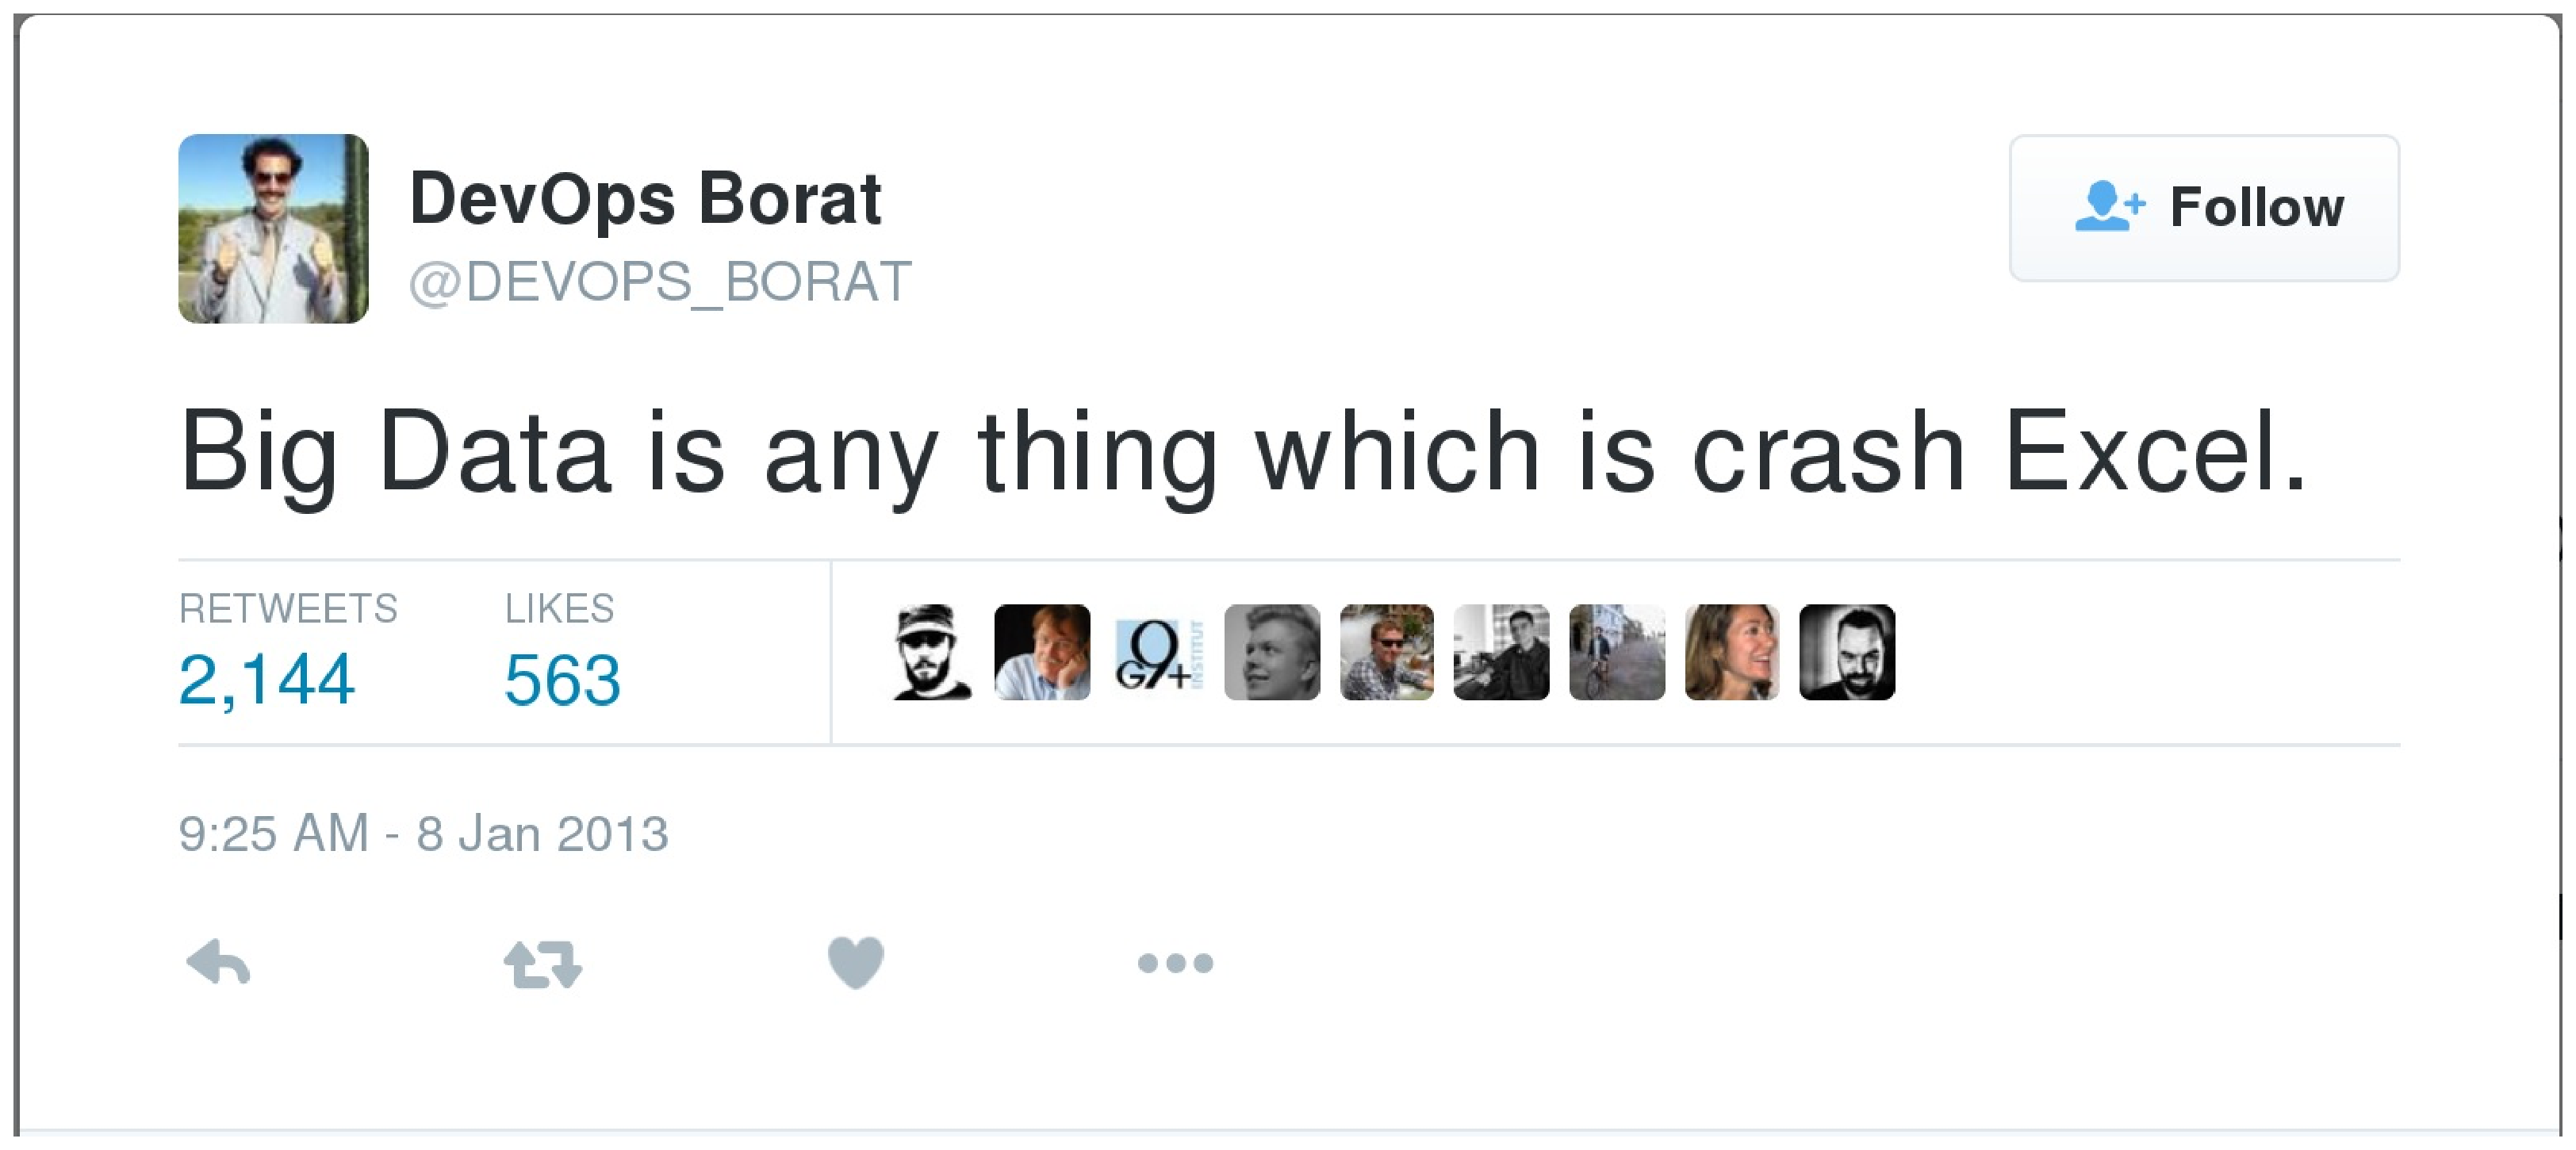
\includegraphics[width=8cm]{./img/borat_big_data.eps}
			\caption{\tiny{Source: https://twitter.com/DEVOPS\_BORAT/status/288698056470315008}}
		\end{figure}
	}
	\visible<3> {
		\begin{itemize}
			\item You can scale up, but sooner or later you'll need to scale out
			\item Need for highly scaleable solution also because of cost effectiveness
		\end{itemize}
	}
\end{frame}

\begin{frame}
	\frametitle{Some of Big data challenges}
	\begin{itemize}
		\item Analysis run on top of the huge amount of data
		\item Sometimes need to pre-process (semi)structured data
		\item Cloud achitecture - everything is ephemeral
	\end{itemize}

	\visible<2,3> {	
		\vspace{0.5cm}
		\textbf{How these challenges are usually addressed:}
			\begin{itemize}
			\item Data replication
			\item Map-reduce model
		\end{itemize}
	}
	
	\visible<3> {
		\vspace{0.5cm}
		\textbf{Probably the most popular implementation:}
		\begin{itemize}
			\item
				\begin{figure}
					
\includegraphics[width=3cm, left]{./img/hadoop-logo.eps}
				\end{figure}	
		\end{itemize}
	}

\end{frame}

\begin{frame}
	\frametitle{Speeding up!}
	\begin{columns}
	\column{0.38\textwidth}
		\begin{figure}
			\centering
			
\includegraphics[width=4cm]{./img/spark-logo.eps}
		\end{figure}
	\column{0.6\textwidth}
		\begin{itemize}
			\item Data grid platform, written in Java
		\end{itemize}
	\end{columns}

	\begin{columns}
	\column{0.6\textwidth}
		\begin{itemize}
			\item For some type of jobs (e.g. iterative alorithms) substential speed up
			\item Speed up of one, sometimes even two orders of magnitude
		\end{itemize}
	\column{0.38\textwidth}
	  \begin{figure}
			\centering
			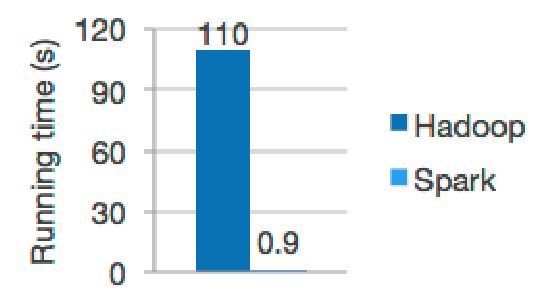
\includegraphics[width=4cm]{./img/hadoop_vs_spark.eps}
			\caption{\tiny{Logistic regression (an ML algorithm for classification) in Hadoop and Spark\newline Source: http://spark.apache.org/}}
		\end{figure}
	\end{columns}
\end{frame}
	
% \begin{frame}
% 	\frametitle{Why caching}
% 	\begin{figure}
% 		\centering
% 		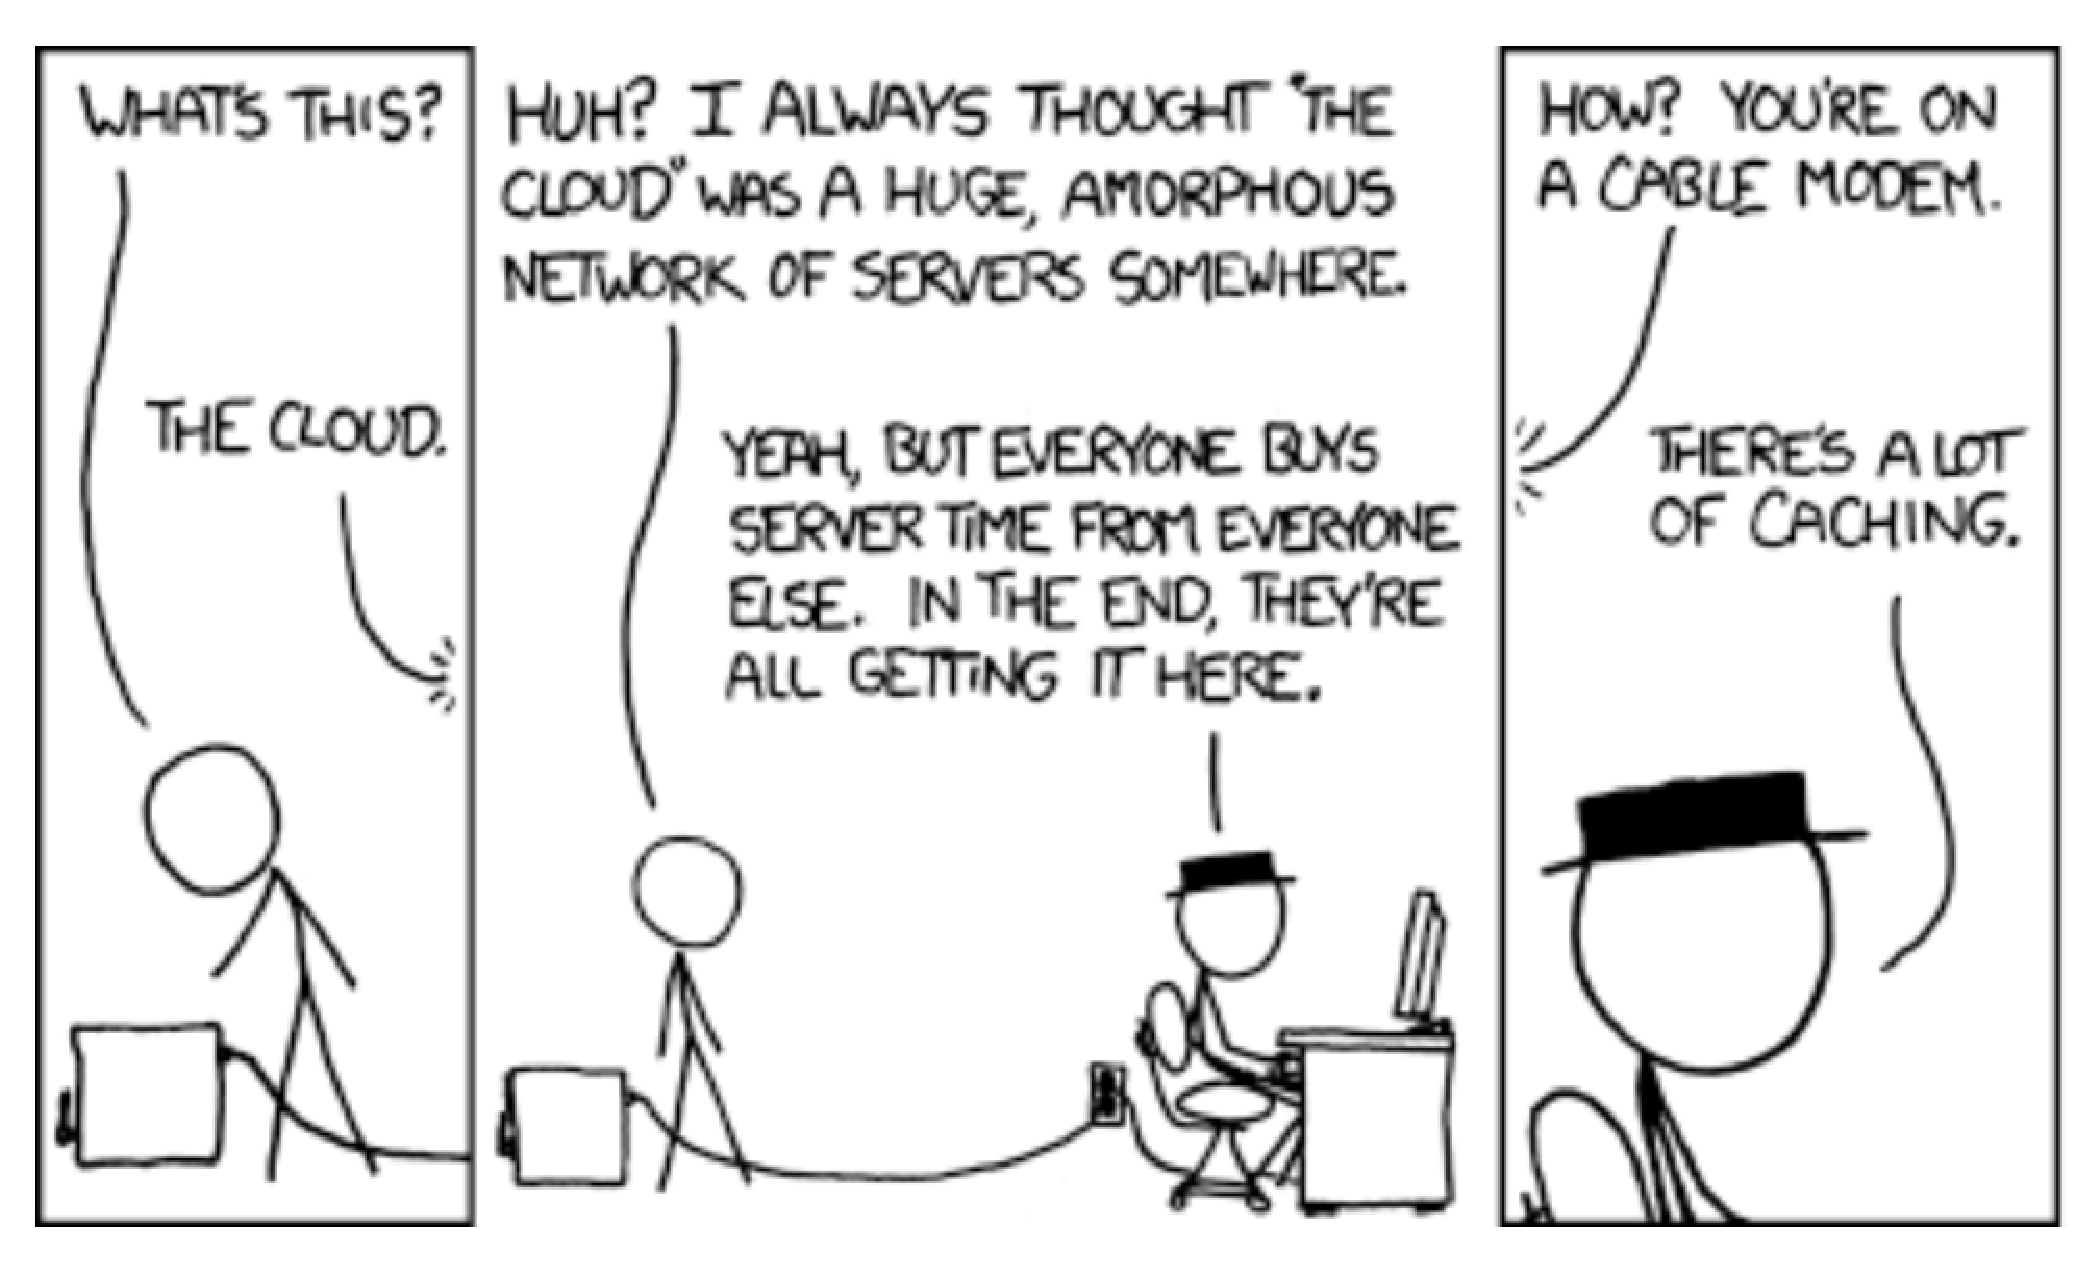
\includegraphics[width=12cm]{./img/xkcd_908.eps}
% 		\caption{\tiny{Source: Part of \href{http://xkcd.com/908/}{xkcd \#908}}}
% 	\end{figure}
% \end{frame}


\begin{frame}
	\frametitle{Demo}
% 	\centering
% 	\huge{\textbf{Demo}} \\
% 	\vspace{1cm}
	\textbf{Infinispan integration with Apache Spark} \\
	\small{\textbf{Temperature}}
% 	\begin{figure}
% 		\centering
% 		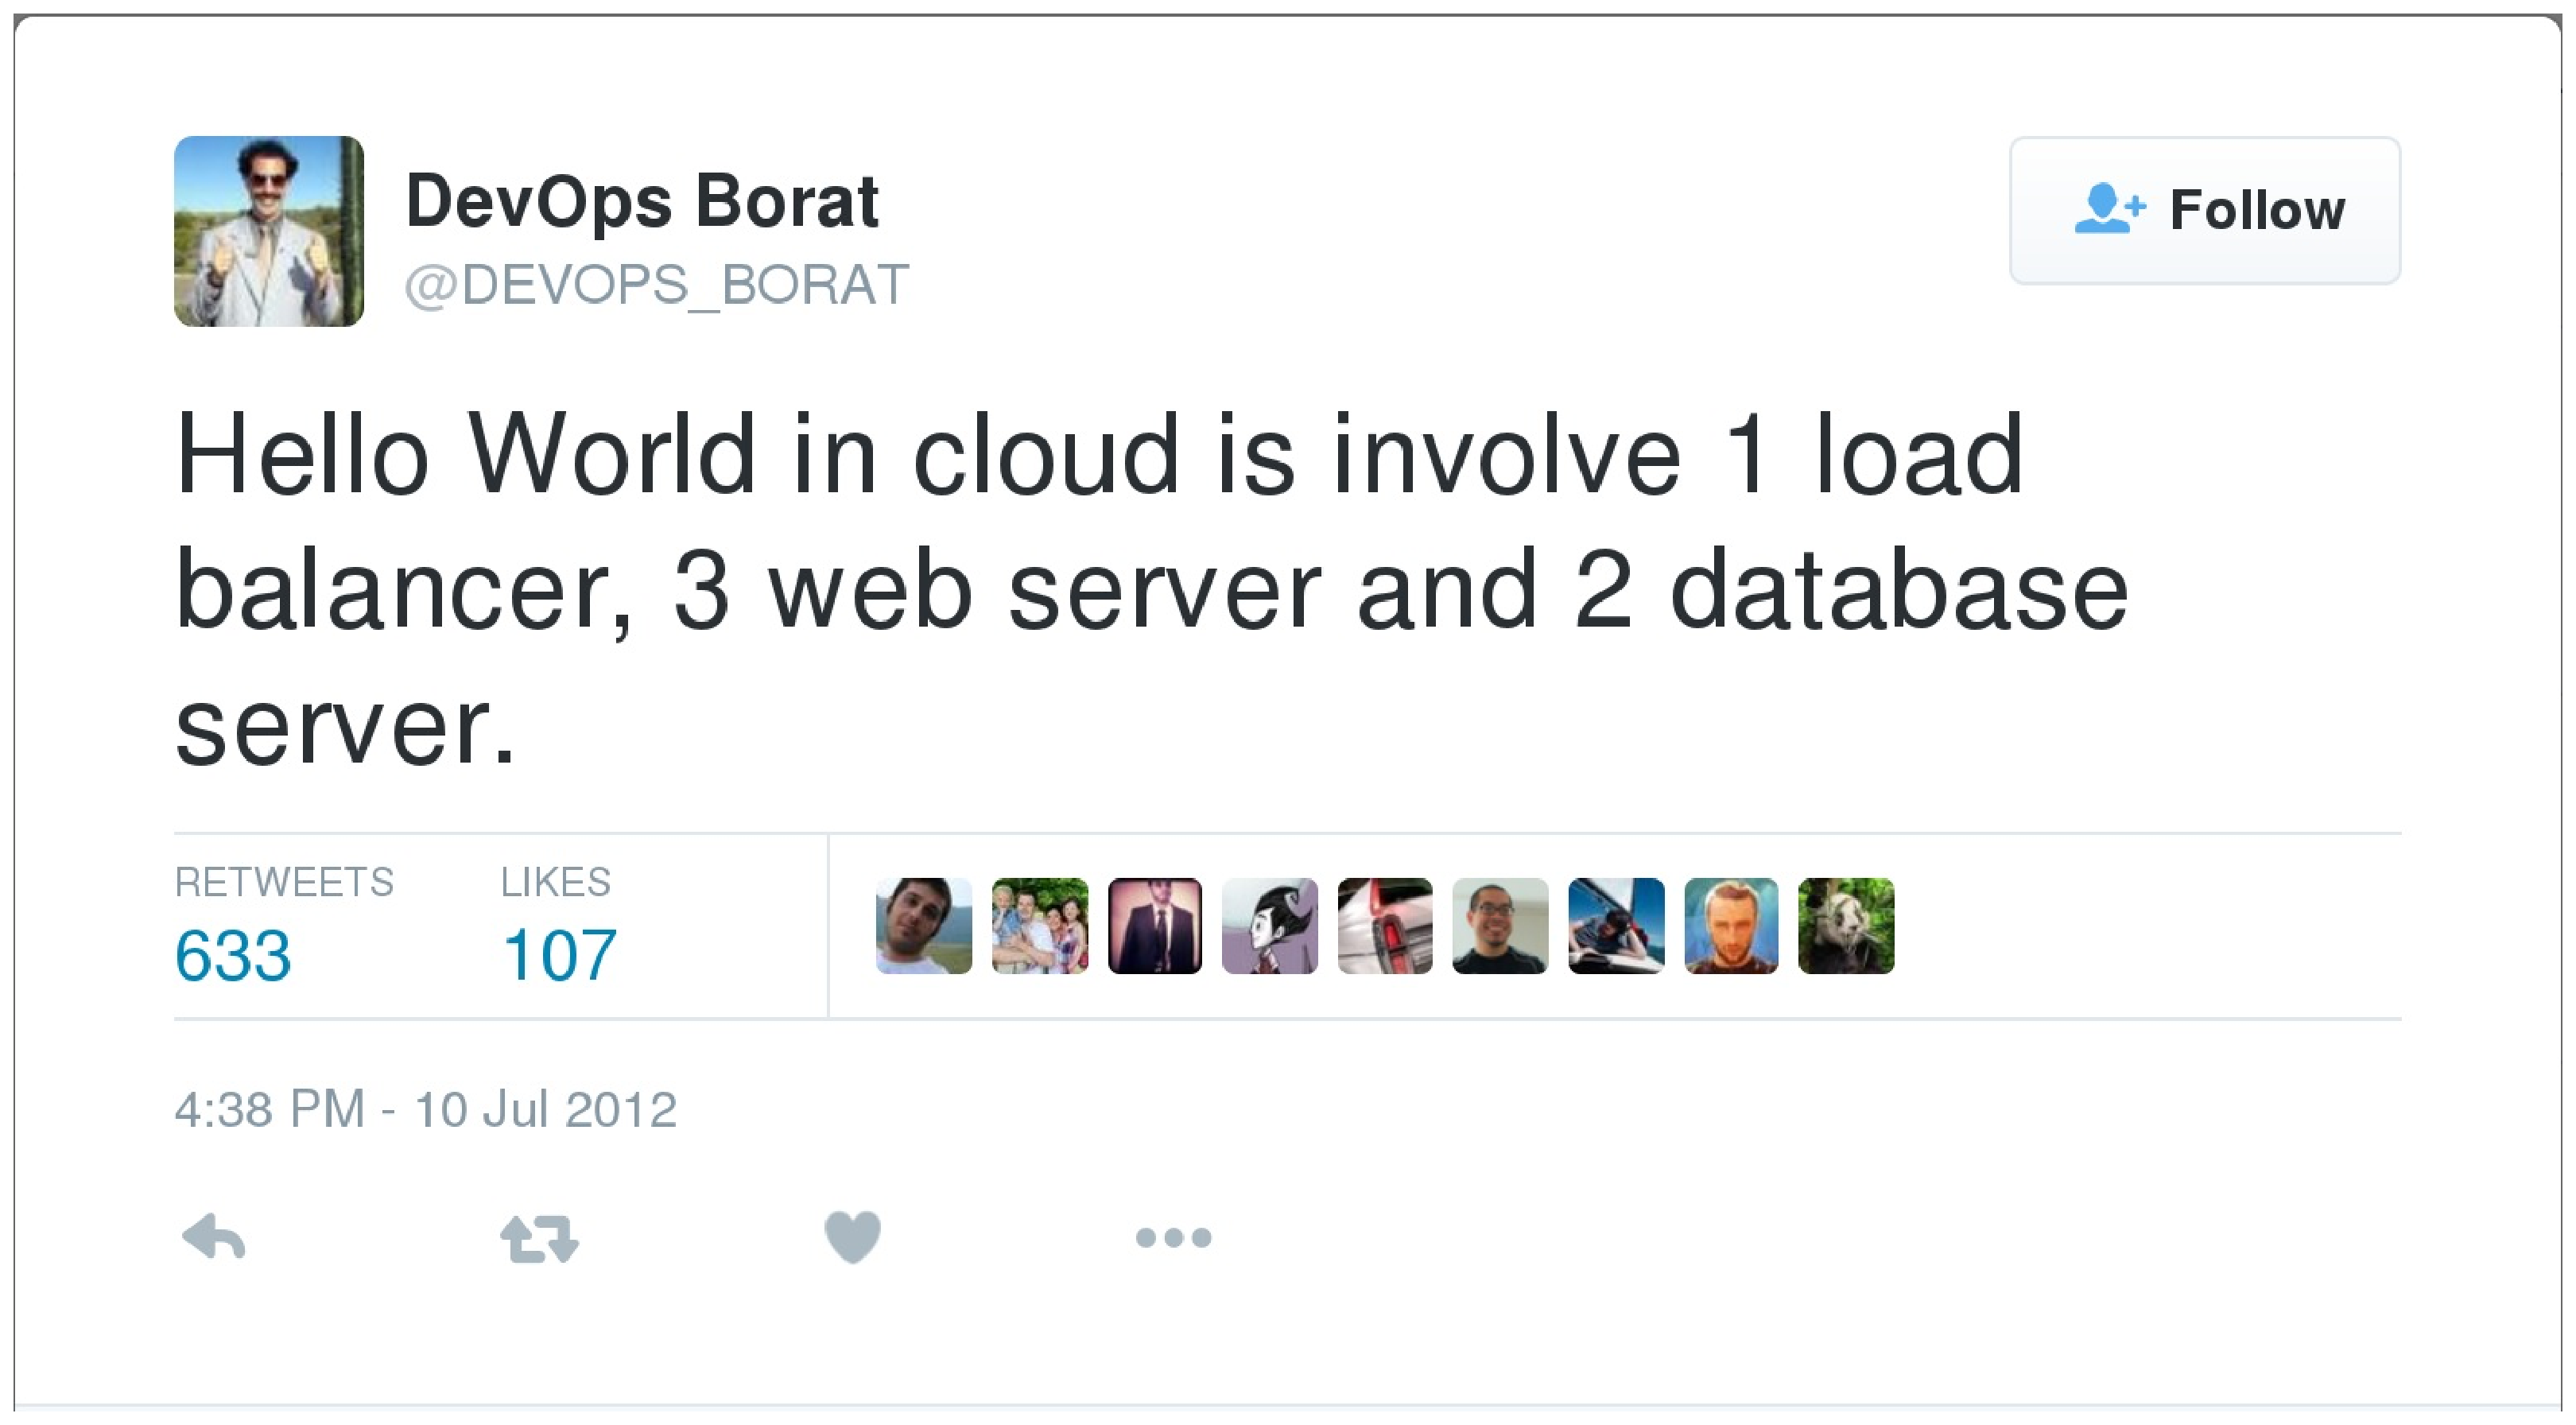
\includegraphics[width=7cm]{./img/borat_hello_world.eps}
% 		\caption{\tiny{Source: https://twitter.com/DEVOPS\_BORAT/status/222837225921060864}}
% 	\end{figure}
\end{frame}

\begin{frame}
	\frametitle{Demo - Hello world}
	\begin{figure}
		\centering
		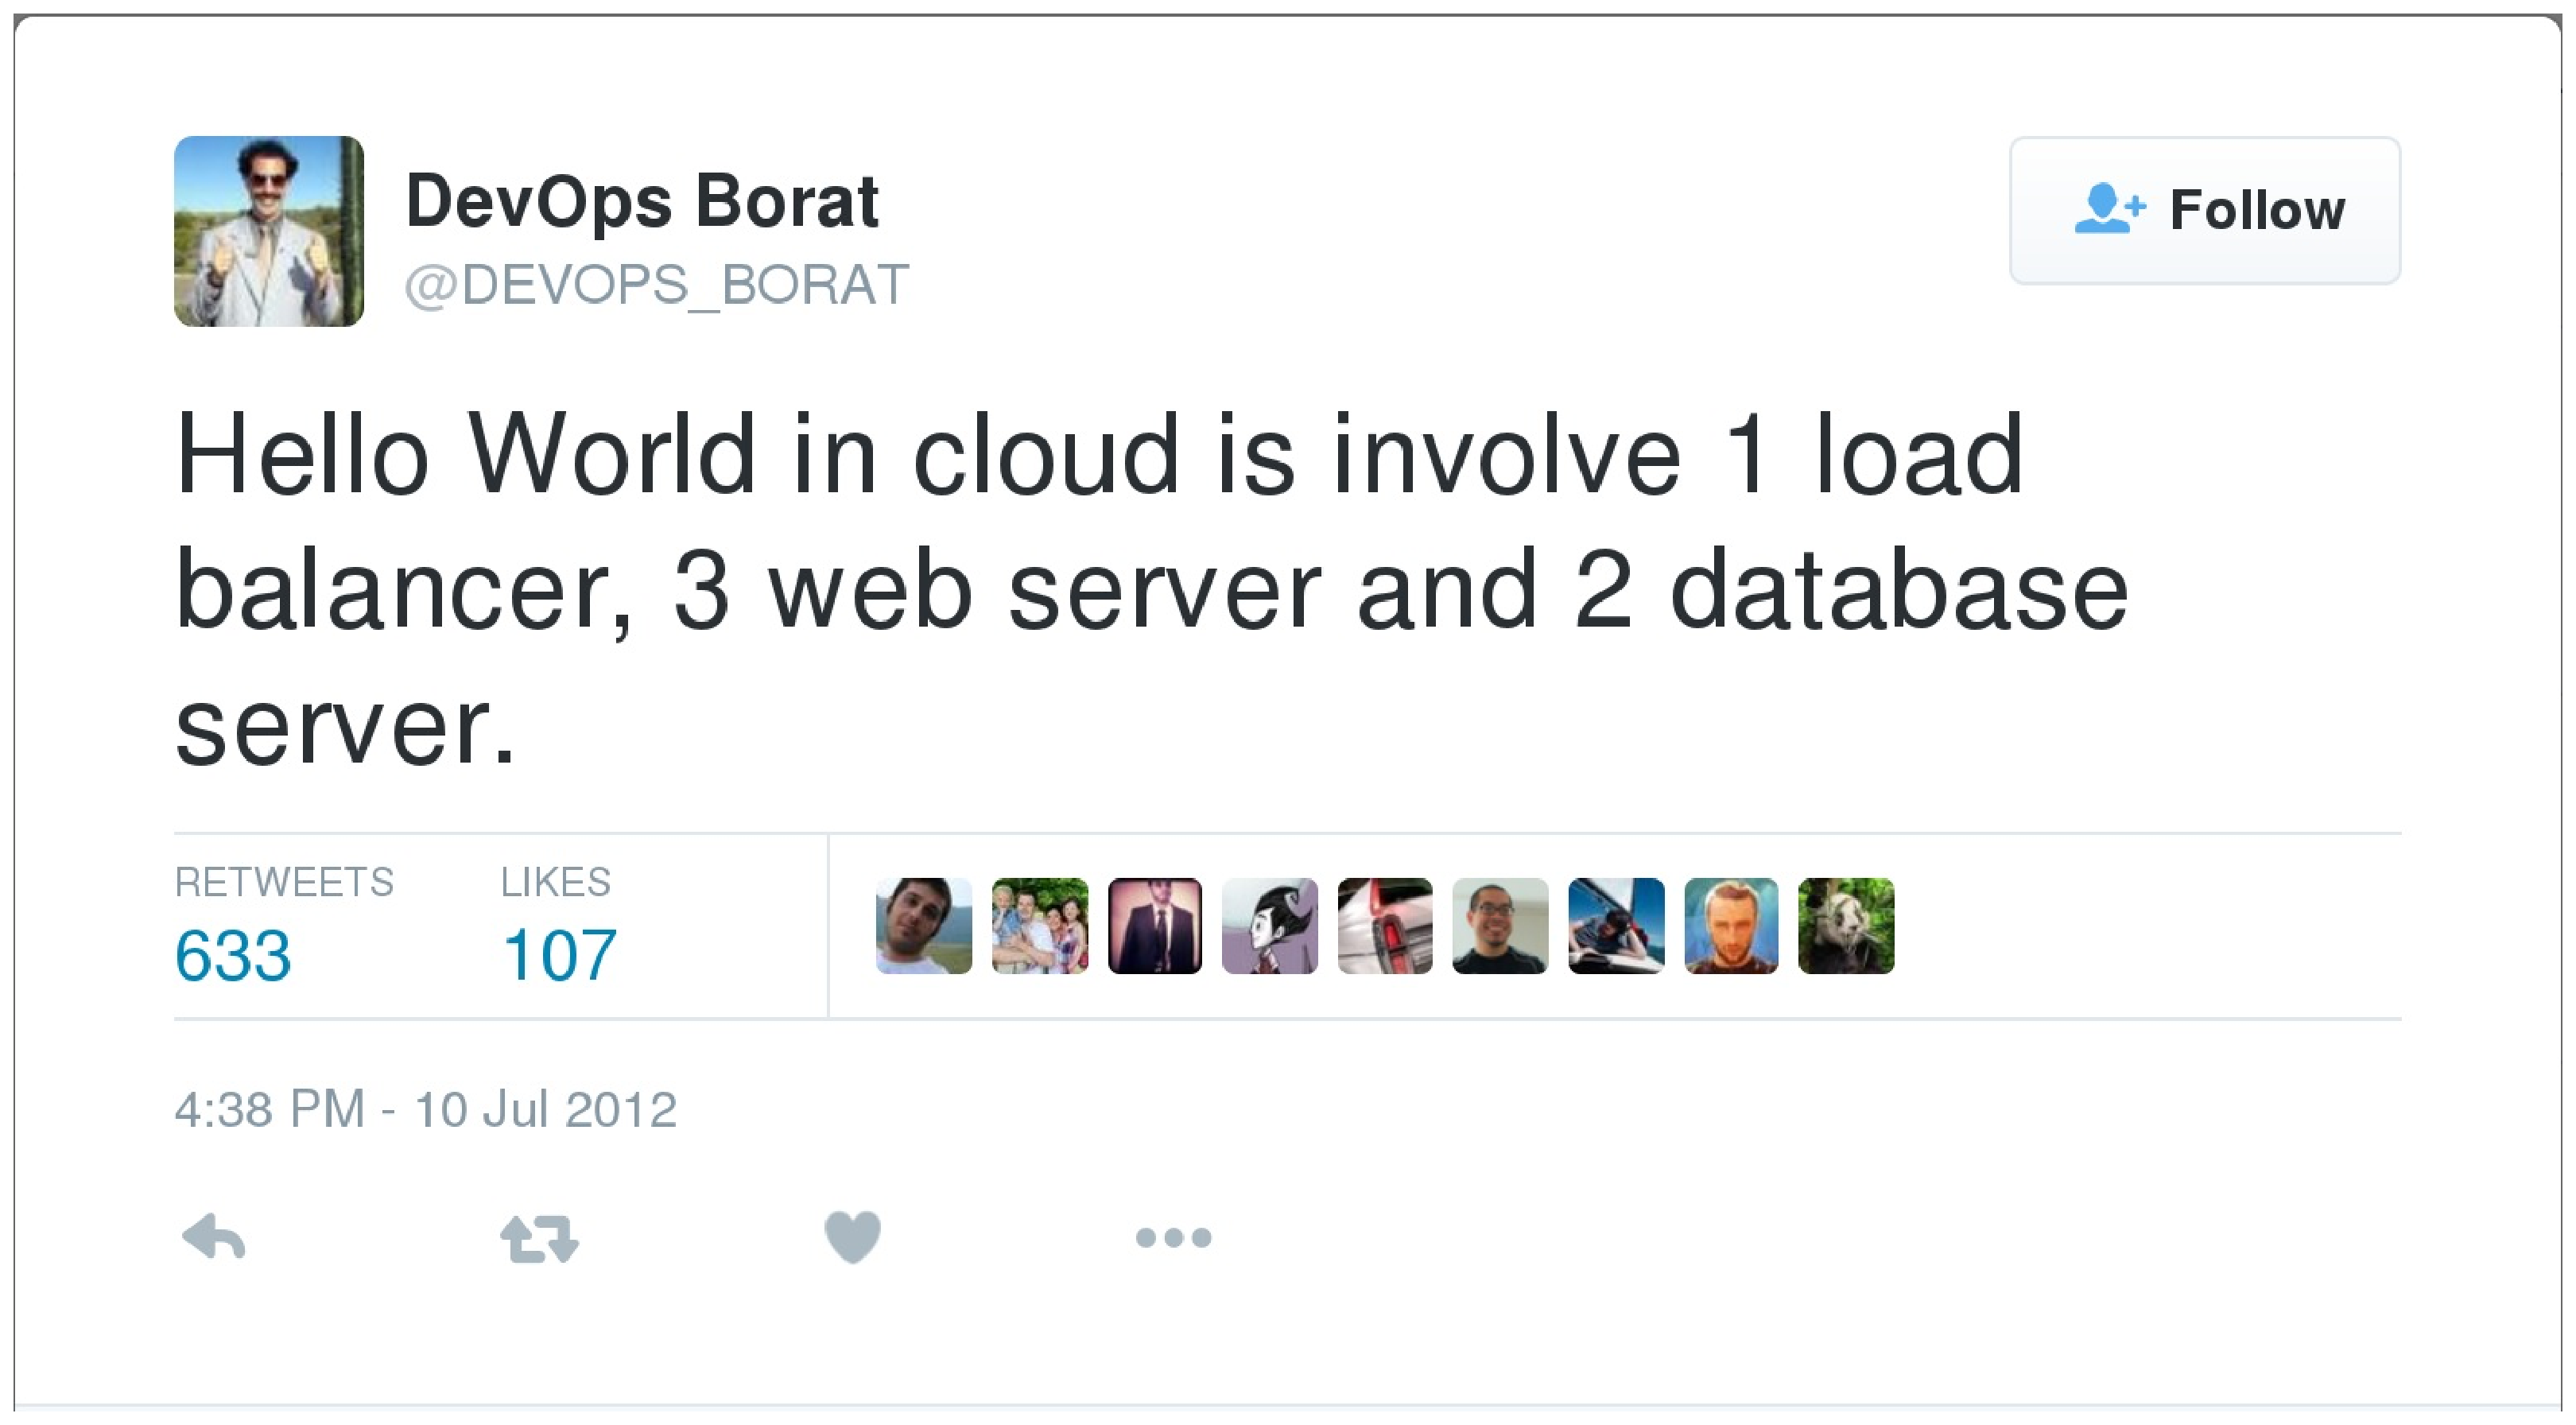
\includegraphics[width=7cm]{./img/borat_hello_world.eps}
		\caption{\tiny{Source: https://twitter.com/DEVOPS\_BORAT/status/222837225921060864}}
	\end{figure}
	
	\begin{itemize}
	 \item One Infinispan server for storing incomming data and results
	 \item One app randomly generating place and temperature (simulating e.g. network of temperature sensors)
	 \item Spark streaming analyzing data 
	 \item Client app showing result data when they arrive
	\end{itemize}
\end{frame}

\begin{frame}
	\frametitle{Summary}
	\begin{itemize}
	 \item 
	\end{itemize}
\end{frame}

\begin{frame}
	\begin{figure}
		\centering
		
\includegraphics[width=2.5cm]{./img/infinispan8.eps}
	\end{figure}
	\centering
	\large{\color{blue}{\url{http://infinispan.org/}}} \\
	\vspace{1cm}
	\huge{\textbf{Thank you for your attention!}} \\
	\vspace{1cm}
	\huge{\textbf{Questions?}}
\end{frame}


\end{document}